\documentclass[12pt,a4paper]{article}
%\usepackage{xcolor} \pagecolor[rgb]{0.5,0.5,0.5} \color[rgb]{1,1,1}
%\usepackage[utf8]{inputenc}
\usepackage[shortlabels]{enumitem}
%\usepackage{bm}
\usepackage{mathrsfs}
\usepackage{amsmath}
\usepackage{amssymb}
\usepackage{hyperref}
\usepackage{graphicx}
\usepackage{pgf, tikz, amsmath, amsfonts}          
\usetikzlibrary{arrows, automata, positioning}

\begin{document}
\title{Solutions to BDA Assignment 2,
 2020/2021 Semester 2}
\author{Theodore Ladas, s2124289}
\date{\today}
\maketitle

This report contains the results from the exploration and modeling of two distrinct statistical problems. The first problem is about modeling the number of earthquakes in Scotland, between 1900 and 2020 from a list of various covariates. 

\noindent\textbf{1)}
\begin{enumerate}[(a)]
\item
Explanation: In this part, an explanatory data analysis is being conducted, in order to gain some initial insight on the dataset. Afterwards, it is assumed that number of earthquakes in Scotland comes from a Poisson distribution with unknown mean parameter $\mu_i$   which is proportional to the number of nonScot earthquakes, namely, 
$\mu_i=\lambda * eartrUK_i$, with the default log link. 

Results:
On \autoref{EDA1} we see a correlation plot, as well as three regressions. On the correlation plot, some things are expected, for example there is a large negative linear correlation between the earthquakes in Scotland \textit{dist} variable, which represents the distance (in miles) of the nearest "nonScot" earthquake to the Scottish border. However we also see a similarly large correalation with decade, indicating that there are less eathquakes in Scotland today, which can be explored further. Lastly, we can also see some problematic regression coefficients between the variables \textit{nrUK4.5}, the number of "nonScot" earthquakes with a magnitude (ML) greater or equal 4.5 and \textit{MLrUK} the average magnitude of "nonScot" earthquakes with $MLrUK > 4$. This suggests that a default logistic regression problem where both of these covariates are present, will have to be very carefully interpreted because of the multicolinearity between those two variables. 

\begin{figure}[h]
    \centering
    \includegraphics[width=0.7\linewidth]{figures/Rplot00.pdf}
    \caption{EDA}
    \label{EDA1}
\end{figure}

On the rest three diagrams, the magnitude of the eathquake is represented by the size of the dots, while the variable \textit{nrUK4.5} is represented by the colour of the dots. There are too few datapoints in order to accurately estimate the relationship between each covariate and the target variable. For example, we see a very pronounce negative slope on the diagram between \textit{dist} and \textit{eartScot}, but it this could be caused by the outliers on the $0$ and the $>300$ distance from the Scottish boarder. 

TODO: GENERATE ANOTHER PLOT WITH EARTHUK

All in all the exploratory data analysis yields that there is no clear answer as to what variables are useful, although it is hinted that the variable \textit{eartrUK} could be a logical choice.


\begin{figure}[]
    \centering
    \includegraphics[width=0.6\linewidth]{figures/Rplot01.pdf}
    \caption{Fitted model}
    \label{model1}
\end{figure}

In this section, the results from the logistic regression model are presented. The intercept  of the regression, after unlinking it by using the inverse of the link function (exponentiating) is 0.5238674, while the coefficient of \textit{eartrUK} is 1.2915168. With these coefficients, the expected number of earthquakew in Scotland in the decade of 1970 and in the decade of 1980 are 0.873819 and 1.882442 respectively, where if we round to the nearghrest integer means that there will be 1 and 2 earthquakes in these decades. 

\begin{figure}[]
    \centering
    \includegraphics[width=0.6\linewidth]{figures/Rplot02.pdf}
    \caption{Predictions per decade}
    \label{prediction1}
\end{figure}

In \autoref{model1}, the fitted model is plotted, along with 1 standard deviation (the grey area). We can clearly see that the fit is capturing most of the information, however it might not be flexible enough to predict accurately.  In \autoref{prediction1}, we see the observed and the predicted values per decade. We can observe that even in a simple model as this one, the fitted model predicts correctly within plus or minus one earthquake. However, it is apparent that in order to have a bigger accuracy, a more complex model is needed.


\item
Explanation: In this section, three Bayesian Poisson models using JAGS were used in order to better estimate the earthquakes in Scotland. On the first one, the $\lambda$ parameter was modeled to have a prior distribution of $\lambda \sim Gamma(0.01,0.01)$, on the second one $lambda \sim Gamma(16,20)$ while the third one was chosen to be a hierarchical model with $lambda \sim Gamma(a,b)$, $a \sim Lognormal(\ln(2),\ln(1.64))$ and $b \sim Lognormal(\ln(4),\ln(1.64))$. Those numbers where chosen so that the expected value of  $\lambda$ would be 0.5 and the coefficient of variation of $\lambda$ would also be 0.5.

Results: The way convergence was checked was through the trace plots, the Gelman Rubin statistic and the Autocorelation plots, which are presented in \autoref{trace}, \autoref{Gelman}, and \autoref{acf}.

\begin{figure}[h]
    \centering
    \includegraphics[width=0.6\linewidth]{figures/Rplot03.pdf}
    \caption{Trace plot}
    \label{trace}
\end{figure}

\begin{figure}[h]
    \centering
    \includegraphics[width=0.6\linewidth]{figures/Rplot04.pdf}
    \caption{Gelman-Rubin plot}
    \label{Gelman}
\end{figure}

\begin{figure}[h]
    \centering
    \includegraphics[width=0.6\linewidth]{figures/Rplot05.pdf}
    \caption{ACF plot}
    \label{acf}
\end{figure}

These are the ways all the Markov chain Monte Carlo chains have beed checked for convergence in this assignment.

The results are that the expectation for $\log(\lambda)$ are $0.3821$, $0.5178$, and $0.3852$ respectively for the three models discribed above. The two candidate models are model 1 and model 3, since these have more defused priors, therefore the explore more options. Also, model 3 is more flexible due to it's hierarchical nature, therefore model 3 is the model of choice.


\item
Explanation:

Results:

\item
The DAG for this model is:

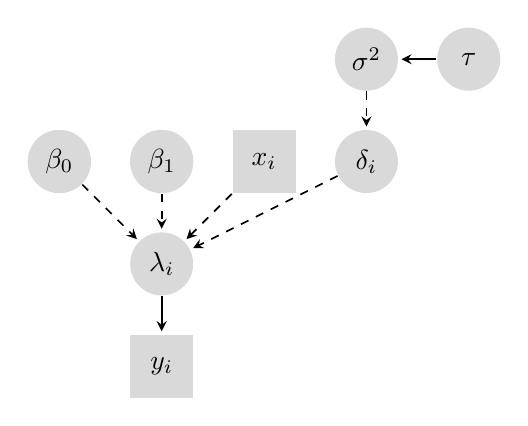
\begin{tikzpicture}[
      > = stealth,                 % arrow head style
      shorten > = 1pt,             % don't touch arrow head to node
      auto, node distance = 1.3cm, % distance between nodes
      semithick                    % thicker arrows
    ]
    
    \tikzstyle{S1}=[      % Defines style for Square 
      fill = black!15,    % Black with transparency 15%
      minimum size = 8mm  
    ]
    
    \tikzstyle{R1}=[      % Defines style for Round 
      circle,             % Changes shape
      fill = black!15,
      minimum size = 8mm
    ]
    
    % DO NOT FORGET ; AT THE END OF EACH SENTENCE!!!
    
    % Definition of the nodes
    % \node[style] (name) [relative_position] {Text};
    % Relative positions: left, right, above, below, above left, etc.
    \node[S1] (y) {$y_{i}$};
    \node[R1] (lambda) [above of=y] {$\lambda_{i}$};
    \node[R1] (beta1) [above of=lambda] {$\beta_1$};
    \node[R1] (beta0) [left of=beta1] {$\beta_0$};
    \node[S1] (x) [right of=beta1] {$x_i$};
    \node[R1] (delta) [right of=x] {$\delta_i$};
    \node[R1] (sigma) [above of=delta] {$\sigma^2$};
    \node[R1] (tau) [right of=sigma] {$\tau$};

    % Definition of the edges
    \path[->] (lambda) edge node {} (y);
    \path[->,dashed] (beta0) edge node {} (lambda);
    \path[->,dashed] (beta1) edge node {} (lambda);
    \path[->,dashed] (delta) edge node {} (lambda);
    \path[->,dashed] (x) edge node {} (lambda);
    
    \path[->,dashed] (sigma) edge node {} (delta);
    \path[->] (tau) edge node {} (sigma);
    

  \end{tikzpicture}
  
In addition to defining the DAG, the model is also built and fitted in the submitted code.

\item
Explanation: Lastly, a model where the earthquakes on Scotland were dependent on the variable $nrUK4.5$ was considered. However, this covariate had missing values. Since the dataset is only 12 datapoints, it is critical to not throw away these potentially valuable datapoints. Instead we can impute the missing values. The way the imputation was performed was via stochastic regression imputation. Essentially, $MLrUK$ was used as an auxiliery variable in the glm model: 

$$\log(\widehat{nrUK4.5})=\widehat{\beta_0}+\widehat{\beta_1}MLrUK$$

After the model was trained, the predictions were created and inserted into the dataset via the predict function.

A second approach into imputing the missing values, was to perform the imputation through JAGS. The model chosen to do this was: 

\begin{verbatim}
model.e2 <- "model{
 # prior
  beta0 ~ dnorm(0,1/5)
  beta1 ~ dnorm(0,1/5)
  
 # Likelihood
  for(i in 1:n) {
      nrUK[i]  ~ dgamma(a.nrUK, b.nrUK)
      log(mu[i]) <- beta0+beta1*(nrUK[i]-mean(nrUK[]))
      eartScot[i] ~ dpois(mu[i])
    } 
  }"
\end{verbatim}

In this model, $nrUK$ is being treaded as a stochastic node that is originated from a gamma distribution. The gamma distribution was chosen, since an only positive and heavily skewed to the left distribution makes sense. The average of the column $nrUK$ when the missing values are removed is around $1$, therefore the $\alpha$ and $\beta$ of the Gamma distribution where chosen to be: $\alpha=6.25$ and $\beta=5.25$, which means that the Gamma distribution has a median value of $1$ and a covariate of variation (or CV) of 0.4. 

\end{enumerate}

\noindent\textbf{2)}
\begin{enumerate}[(a)]

\item
Explanation: In this section, the probability of wildefire in the forests of two Algerian regions: the Bejaia region, located in the Northest of Algeria and the Sidi Bel-abbes region, in the Northwest, are being modeled. In this part an exploratory data analysis is being performed.

Results: In \autoref{EDA2}, we see the four important meteorological variables versus the existance or not of Fire. The lines have been automatically drawn by \textsf{R}, in order to understand the relationship of each covariate to the dependent variable. For example, we see what we expect in the Temperature variable, since as the temperature rises, the probability of fire rises as well. While these lines don't exactly respresent probabilities, there shape is important to gain insight.


\begin{figure}[h]
    \centering
    \includegraphics[width=0.6\linewidth]{figures/Rplot07.pdf}
    \caption{EDA}
    \label{EDA2}
\end{figure}

\begin{figure}[h]
    \centering
    \includegraphics[width=0.6\linewidth]{figures/Rplot08.pdf}
    \caption{Box and Wiskers plots}
    \label{boxplots}
\end{figure}

Secondly, in \autoref{boxplots} the Box and Wiskers plots of the two Regions, stratified by the existance or not of fire are presented. The orange plots are the ones that a fire happened, while the green ones represent the absense of fire. We can see for example, that in general, then the temperature is higher the mean probability of fire is higher. However this needs to be tested further, since we can see that almost all the boxplot (from Q1 to Q3) can be contained in the Inter Quartile Range (IQR) of the green diagrams. That means that this difference in means, might not be stastistically significant. In addition, in the variable RH, which represents daily relative Humidity (\%), The mean probability of Fire in the Sidi Bel-abbes region seems to be significantly lower but the variability of that box plot is extremely large, indicating again that it might not be significant. Lastly, the most important variable seems to be the RainYest (Yesterday's precipitations in $mm/m^2$) variable.

\item
Explanation: A glm Bernouli model with these four covariates has been fitter to predict the probability of Fire. The logit link was used. After unlinkin through the inverse logit function, the coefficients are (Intercept):0.549 TempCels:0.579 RH:0.492 Ws:0.519 RainYest:0.339. 
Lastly, the probability of a fire on the new data was estimated to be: 0.00049. 

\item
The same model was fitted with JAGS this time. In order for the chains to converge, a burnin of 2000, along with 50000 iterations were chosen. Some autocorelation was present with these initial values, therefore, a thining of 100 was selected as well. The coefficints are, (Intercept):0.453 TempCels:0.418 RH:0.508 Ws:0.480 RainYest:0.667 which are similar but not the same as the previous model. The interpretation of the intercept is that there is a 45.3\% probability of a Fire on the average levels of the variables Temperature, RH, Wind speeds and RainYest. As for the rest have the same interpretation and TempCels is going to be used as an example. When TempCels increases by one unit, there is a 4.18\% increase in the probability of Fire in Algeria.

\item
In this section three JAGS models have been fitted, progressivly more complex, which are reported here along the initial values that ensured convergence. 

\begin{verbatim}
model.d1 <- "model{
  # Likelihood
  for(i in 1:n) {
      Fire[i] ~ dbern(mu[i])
      logit(mu[i]) <- -(beta0[j.region[i]] + 
                        beta1*TempCels[i] + 
                        beta2*RH[i] + 
                        beta3*Ws[i] + 
                        beta4*RainYest[i])
  }
  
  # priors for independent intercepts per county
  for(j in 1:J){
    beta0[j] ~ dnorm(0,1/0.1)
  }
  # prior
  beta1 ~ dnorm(0,1/100)
  beta2 ~ dnorm(0,1/100)
  beta3 ~ dnorm(0,1/100)
  beta4 ~ dnorm(0,1/100)
  }"
\end{verbatim}

Model.d1 initial values: 
Initial values for all beta coefficient were set with a zero centered Normal prior and 1 of standard deviation.
\begin{itemize}
\item chains: 5
\item thin: 100
\item iterations: 50000
\item burnin: 7000
\end{itemize}

All the effective sample size are above 2500. 

\begin{figure}[h]
    \centering
    \includegraphics[width=0.6\linewidth]{figures/Rplot09.pdf}
    \caption{Model d1}
    \label{model d1}
\end{figure}

In \autoref{model d1} The posterior expected probabilities of fire in the two Algerian region are plotted.

\begin{verbatim}
model.d2 <- "model{
  # Likelihood
  for(i in 1:n) {
      Fire.rep[i] ~ dbern(mu[i])
      Fire[i] ~ dbern(mu[i])
      logit(mu[i]) <- -(beta0[Region.month.b[i]] + 
                        beta1*TempCels[i] + 
                        beta2*RH[i] + 
                        beta3*Ws[i] + 
                        beta4*RainYest[i] +
                        beta5[j.region[i]]*month.b[i])
  }
  # priors for independent intercepts per county
  for(j in 1:J){
    beta5[j] ~ dnorm(0,1/0.1)
  }
  
  for(k in 1:K){
    beta0[k] ~ dnorm(0,1/0.1)
  }
  
  # prior
  beta1 ~ dnorm(0,1/100)
  beta2 ~ dnorm(0,1/100)
  beta3 ~ dnorm(0,1/100)
  beta4 ~ dnorm(0,1/100)
  }"
\end{verbatim}

Model.d2 initial values: 
Initial values for all beta coefficient were set with a zero centered Normal prior and 1 of standard deviation.
\begin{itemize}
\item chains: 5
\item thin: 100
\item iterations: 50000
\item burnin: 2000
\end{itemize}

All the effective sample size are above 2500. 

\begin{figure}[h]
    \centering
    \includegraphics[width=0.6\linewidth]{figures/Rplot10.pdf}
    \caption{Model d2}
    \label{model d2}
\end{figure}

In \autoref{model d2} The posterior expected probabilities of fire in the two Algerian region are plotted.


\begin{verbatim}
model.d3 <- "model{
  # Likelihood
  for(i in 1:n) {
      Fire.rep[i] ~ dbern(mu[i])
      Fire[i] ~ dbern(mu[i])
      logit(mu[i]) <- -(beta0[region.month[i]] + 
                        beta1*TempCels[i] + 
                        beta2*RH[i] + 
                        beta3*Ws[i] + 
                        beta4*RainYest[i]) +
                        omega[region.month[i]]
  }
  
  # priors for independent intercepts per county
  for(j in 1:J){
    beta0[j] ~ dnorm(0, 1/0.1)
    omega[j] ~ dnorm(0, 1/omega.sigma2)
  }
  # prior
  beta1 ~ dnorm(0,1/100)
  beta2 ~ dnorm(0,1/100)
  beta3 ~ dnorm(0,1/100)
  beta4 ~ dnorm(0,1/100)
  omega.sigma2 ~ dgamma(0.01,0.01)
}"
\end{verbatim}

Model.d3 initial values: 
Initial values for all beta coefficient were set with a zero centered Normal prior and 1 of standard deviation.
\begin{itemize}
\item chains: 5
\item thin: 100
\item iterations: 50000
\item burnin: 2000
\end{itemize}


All the effective sample size are above 2500. 

\begin{figure}[h]
    \centering
    \includegraphics[width=0.6\linewidth]{figures/Rplot11.pdf}
    \caption{Model e1}
    \label{model d3}
\end{figure}

In \autoref{model d3} The posterior expected probabilities of fire stratified by the four monhts in the two Algerian Regions is plotted.
This models has also been fitted with INLA, however the results are not the same. This means that something is not correct on the setting of the INLA model.

\item

In this section posterior predictive checks are being presented. 50000 posterior predicitve samples have been generated from the posterior predictive distribution of models d2, d3 and e1. Then the sums of fires per Region per month have been calculated in these posterior samples. Since we can also calculate the sums of fire pre region per month on the original sample, then, we can plot the distribution of this statistic (called \textit{total fires}) and the observed values in \autoref{final}. 

\begin{figure}[h]
    \centering
    \includegraphics[width=1\linewidth]{figures/Rplot12.pdf}
    \caption{Simulated Fires}
    \label{final}
\end{figure}

The table of the probabilities of observing a proportion of wildfires for each region and month that is more extreme than those observed in the actual dataset is also being reported here. More extreme means, bigger value in the \textit{total fires} column.

\begin{table}
\centering
\begin{tabular}{|l|lll|} 
\hline
\multicolumn{1}{|l}{Model} & Region & Month & Probability                                        \\ 
\hline
d2                         & B      & 6     & 0.24326                                            \\
d2                         & B      & 7     & 0.57966                                            \\
d2                         & B      & 8     & 0.34038                                            \\
d2                         & B      & 9     & 0.60928                                            \\
d2                         & S      & 6     & 0.87126                                            \\
d2                         & S      & 7     & 0.18758                                            \\
d2                         & S      & 8     & 0.37692                                            \\
d2                         & S      & 9     & 0.10148                                            \\
d3                         & B      & 6     & 0.28778                                            \\
d3                         & B      & 7     & 0.53380                                            \\
d3                         & B      & 8     & 0.39554                                            \\
d3                         & B      & 9     & 0.53670                                            \\
d3                         & S      & 6     & 0.67466                                            \\
d3                         & S      & 7     & 0.13770                                            \\
d3                         & S      & 8     & 0.26356                                            \\
d3                         & S      & 9     & 0.10782                                            \\
e1                         & B      & 6     & 0.20640                                            \\
e1                         & B      & 7     & 0.34184                                            \\
e1                         & B      & 8     & 0.38944                                            \\
e1                         & B      & 9     & 0.22506                                            \\
e1                         & S      & 6     & 0.34068                                            \\
e1                         & S      & 7     & 0.25394                                            \\
e1                         & S      & 8     & 0.40288                                            \\
e1                         & S      & 9     & 0.16360                                            \\
\hline
\end{tabular}
\end{table}

Lastly, the DIC scores for d2, d3, and e1 are 237.5, 235, 190.2 respectively. Since model e1 has a lower DIC score, that means that it is the prefered model.

The last question is about finding the hyperparameters of a prior for the parameter DMC where we elicit the information from a domain expert. 
\end{enumerate}
\end{document}